\documentclass[tikz, border=16pt]{standalone}
\usepackage{tikz}
\usepackage{amsmath}
\usetikzlibrary{arrows.meta, backgrounds, calc}

%% Layout (all y in cm, x centred at 0, frames ±7 cm wide)
%%
%%  SB3        : centre y=22,  h=1.2  → N=22.6  S=21.4
%%  gap-1 arrows                         21.4 → 20.5  (0.9 cm)
%%  VecEnv     : centre y=18.2, h=4.6 → N=20.5  S=15.9
%%  gap-2 arrows                         15.9 → 14.8  (1.1 cm)
%%  TCEnv      : centre y= 9.8, h=10  → N=14.8  S= 4.8
%%  gap-3 arrows                          4.8 →  3.1  (1.7 cm)
%%  SUMO       : centre y= 2.5, h=1.2 → N= 3.1  S= 1.9
%%  Legend     : y=1.4

\begin{document}
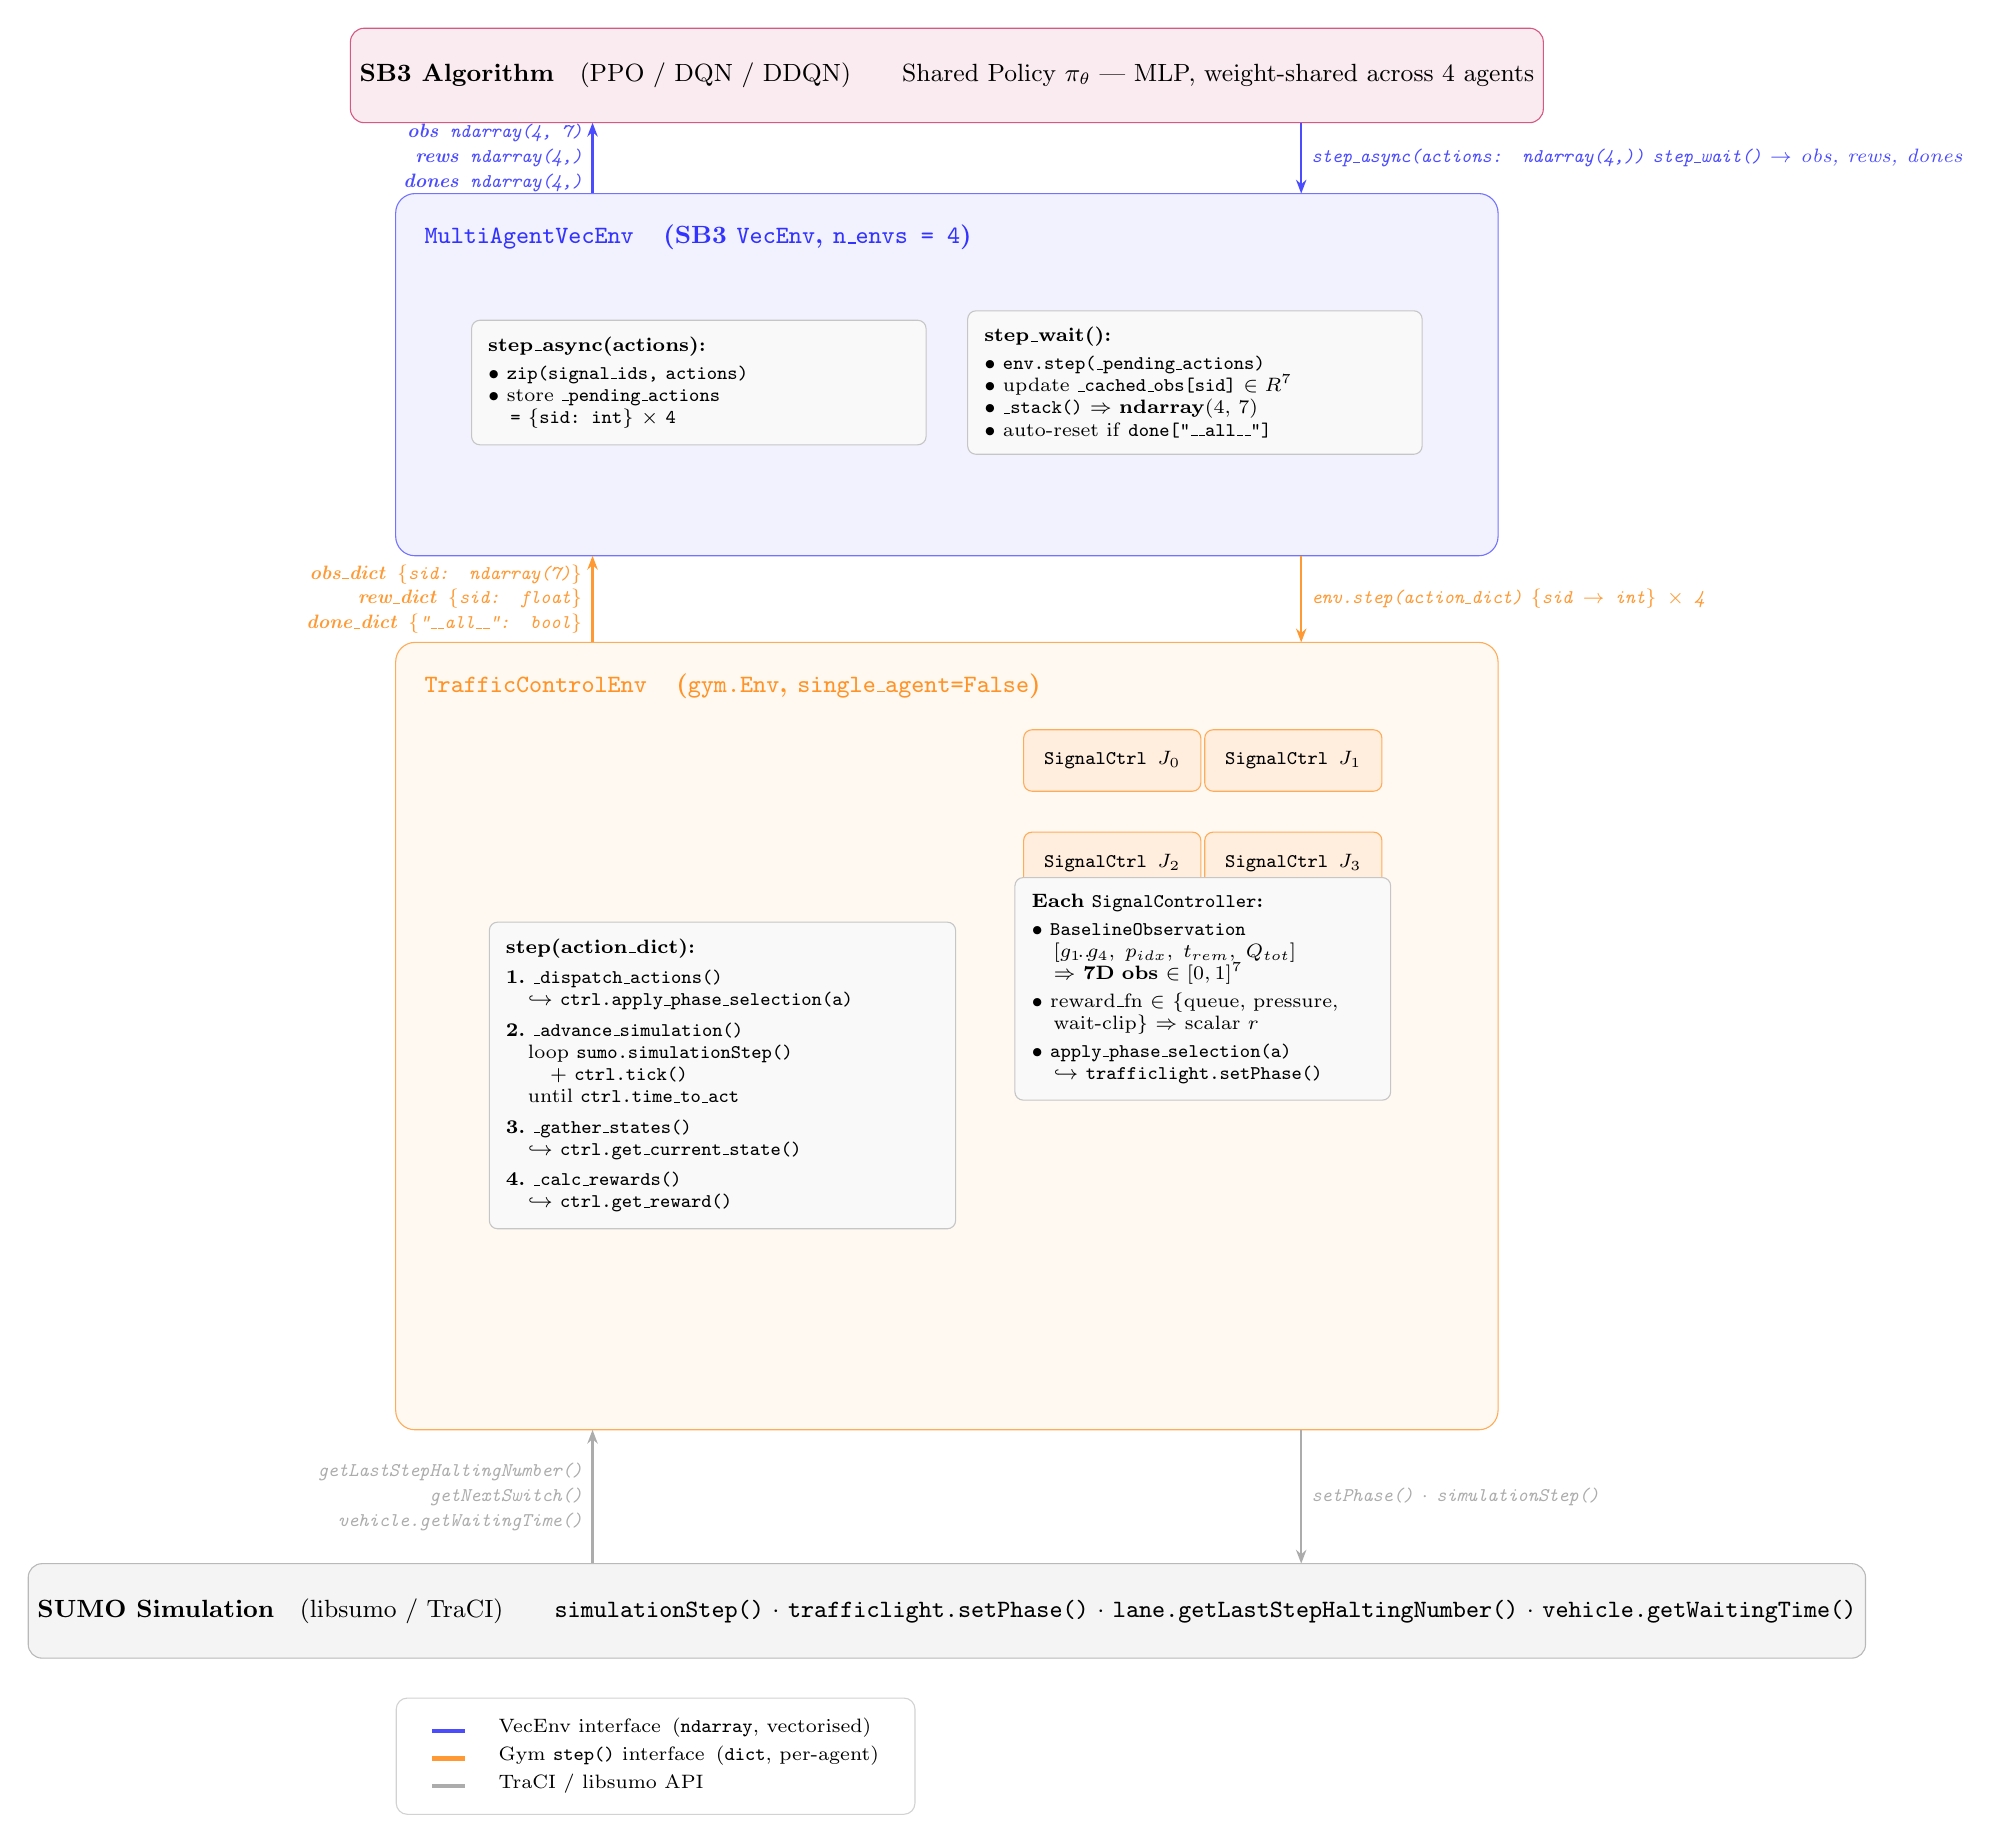
\begin{tikzpicture}[
    ibox/.style={rectangle, draw=gray!45, rounded corners=3pt, fill=gray!5,
                 font=\scriptsize, inner sep=6pt, text width=#1, align=left},
    scbox/.style={rectangle, draw=orange!65, rounded corners=3pt, fill=orange!13,
                  font=\scriptsize\ttfamily, inner sep=4pt,
                  minimum width=2.25cm, minimum height=0.78cm, text centered},
    arr/.style={-{Stealth[length=5pt]}, thick},
    lbl/.style={font=\scriptsize\itshape},
]

%% ══════════════════════════════════════════════════════
%% LAYER 0 — SB3 Algorithm
%% ══════════════════════════════════════════════════════
\node[rectangle, draw=purple!65, rounded corners=5pt, fill=purple!8,
      minimum width=14cm, minimum height=1.2cm, font=\small]
     (sb3) at (0,22) {
    \textbf{SB3 Algorithm}\quad(PPO / DQN / DDQN)\qquad
    Shared Policy $\pi_\theta$ — MLP, weight-shared across 4 agents
};

%% ── gap-1 arrows (0.9 cm gap, y = 20.5 … 21.4) ──────
\draw[arr, blue!70] (4.5, 21.4) --
    node[right, lbl]{
        \texttt{step\_async(actions: \textbf{ndarray}(4,))}\\[1pt]
        \texttt{step\_wait()} $\to$ obs,\ rews,\ dones}
    (4.5, 20.5);

\draw[arr, blue!70] (-4.5, 20.5) --
    node[left, lbl, align=right]{
        \textbf{obs}\enspace\texttt{ndarray(4, 7)}\\[1pt]
        \textbf{rews}\enspace\texttt{ndarray(4,)}\\[1pt]
        \textbf{dones}\enspace\texttt{ndarray(4,)}}
    (-4.5, 21.4);

%% ══════════════════════════════════════════════════════
%% LAYER 1 — MultiAgentVecEnv
%% Frame: centre (0, 18.2), 14×4.6 cm  → N=20.5 S=15.9
%% ══════════════════════════════════════════════════════
\node[rectangle, draw=blue!55, rounded corners=7pt, fill=blue!5,
      minimum width=14cm, minimum height=4.6cm, inner sep=0pt]
     (vecframe) at (0,18.2) {};

\node[font=\small\bfseries, text=blue!80, anchor=north west]
     at ($(vecframe.north west)+(0.25,-0.28)$)
     {\texttt{MultiAgentVecEnv}\quad(SB3 \texttt{VecEnv},\ \texttt{n\_envs = 4})};

\node[ibox=5.35cm] at (-3.15, 18.1) {
    \textbf{step\_async(actions):}\\[2pt]
    $\bullet$\ \texttt{zip(signal\_ids, actions)}\\
    $\bullet$\ store \texttt{\_pending\_actions}\\
    \quad\texttt{= \{sid: int\} $\times$ 4}
};

\node[ibox=5.35cm] at (3.15, 18.1) {
    \textbf{step\_wait():}\\[2pt]
    $\bullet$\ \texttt{env.step(\_pending\_actions)}\\
    $\bullet$\ update \texttt{\_cached\_obs[sid]} $\in\mathbb{R}^7$\\
    $\bullet$\ \texttt{\_stack()} $\Rightarrow$ \textbf{ndarray}(4, 7)\\
    $\bullet$\ auto-reset if \texttt{done["\_\_all\_\_"]}
};

%% ── gap-2 arrows (1.1 cm gap, y = 14.8 … 15.9) ──────
\draw[arr, orange!80] (4.5, 15.9) --
    node[right, lbl]{
        \texttt{env.step(action\_dict)}\\[1pt]
        \texttt{\{sid $\to$ int\} $\times$ 4}}
    (4.5, 14.8);

\draw[arr, orange!80] (-4.5, 14.8) --
    node[left, lbl, align=right]{
        \textbf{obs\_dict}\enspace\texttt{\{sid: ndarray(7)\}}\\[1pt]
        \textbf{rew\_dict}\enspace\texttt{\{sid: float\}}\\[1pt]
        \textbf{done\_dict}\enspace\texttt{\{"\_\_all\_\_": bool\}}}
    (-4.5, 15.9);

%% ══════════════════════════════════════════════════════
%% LAYER 2 — TrafficControlEnv
%% Frame: centre (0, 9.8), 14×10 cm  → N=14.8 S=4.8
%% ══════════════════════════════════════════════════════
\node[rectangle, draw=orange!65, rounded corners=7pt, fill=orange!5,
      minimum width=14cm, minimum height=10.0cm, inner sep=0pt]
     (tceframe) at (0,9.8) {};

\node[font=\small\bfseries, text=orange!85, anchor=north west]
     at ($(tceframe.north west)+(0.25,-0.28)$)
     {\texttt{TrafficControlEnv}\quad(\texttt{gym.Env},\ \texttt{single\_agent=False})};

%% left column — step() chain
\node[ibox=5.5cm] at (-2.85, 9.3) {
    \textbf{step(action\_dict):}\\[3pt]
    \textbf{1.}\ \texttt{\_dispatch\_actions()}\\
    \quad $\hookrightarrow$ \texttt{ctrl.apply\_phase\_selection(a)}\\[3pt]
    \textbf{2.}\ \texttt{\_advance\_simulation()}\\
    \quad loop \texttt{sumo.simulationStep()}\\
    \quad\quad + \texttt{ctrl.tick()}\\
    \quad until \texttt{ctrl.time\_to\_act}\\[3pt]
    \textbf{3.}\ \texttt{\_gather\_states()}\\
    \quad $\hookrightarrow$ \texttt{ctrl.get\_current\_state()}\\[3pt]
    \textbf{4.}\ \texttt{\_calc\_rewards()}\\
    \quad $\hookrightarrow$ \texttt{ctrl.get\_reward()}
};

%% right column — 4 SignalControllers (2×2 grid)
\node[scbox] at (2.1, 13.3) {\texttt{SignalCtrl $J_0$}};
\node[scbox] at (4.4, 13.3) {\texttt{SignalCtrl $J_1$}};
\node[scbox] at (2.1, 12.0) {\texttt{SignalCtrl $J_2$}};
\node[scbox] at (4.4, 12.0) {\texttt{SignalCtrl $J_3$}};

%% right column — SignalController internals
\node[ibox=4.35cm] at (3.25, 10.4) {
    \textbf{Each \texttt{SignalController}:}\\[2pt]
    $\bullet$\ \texttt{BaselineObservation}\\
    \quad $[g_1\!..\!g_4,\;p_{idx},\;t_{rem},\;Q_{tot}]$\\
    \quad $\Rightarrow$ \textbf{7D obs} $\in [0,1]^7$\\[2pt]
    $\bullet$\ reward\_fn $\in$ \{queue, pressure,\\
    \quad wait-clip\} $\Rightarrow$ scalar $r$\\[2pt]
    $\bullet$\ \texttt{apply\_phase\_selection(a)}\\
    \quad $\hookrightarrow$ \texttt{trafficlight.setPhase()}
};

%% ── gap-3 arrows (1.7 cm gap, y = 3.1 … 4.8) ────────
\draw[arr, gray!65] (4.5, 4.8) --
    node[right, lbl]{
        \texttt{setPhase()} $\cdot$ \texttt{simulationStep()}}
    (4.5, 3.1);

\draw[arr, gray!65] (-4.5, 3.1) --
    node[left, lbl, align=right]{
        \texttt{getLastStepHaltingNumber()}\\[1pt]
        \texttt{getNextSwitch()}\\[1pt]
        \texttt{vehicle.getWaitingTime()}}
    (-4.5, 4.8);

%% ══════════════════════════════════════════════════════
%% LAYER 3 — SUMO Simulation
%% ══════════════════════════════════════════════════════
\node[rectangle, draw=gray!55, rounded corners=5pt, fill=gray!9,
      minimum width=14cm, minimum height=1.2cm, font=\small]
     (sumo) at (0,2.5) {
    \textbf{SUMO Simulation}\quad(libsumo / TraCI)\qquad
    \texttt{simulationStep()} $\cdot$
    \texttt{trafficlight.setPhase()} $\cdot$
    \texttt{lane.getLastStepHaltingNumber()} $\cdot$
    \texttt{vehicle.getWaitingTime()}
};

%% ══════════════════════════════════════════════════════
%% LEGEND
%% ══════════════════════════════════════════════════════
\node[rectangle, draw=gray!35, rounded corners=4pt, fill=white,
      inner sep=7pt, font=\scriptsize, anchor=north west]
     at (-7, 1.4) {
    \begin{tabular}{ll}
        \textcolor{blue!70}{\rule{12pt}{1.5pt}}   &
            VecEnv interface\enspace(\texttt{ndarray}, vectorised)\\[2pt]
        \textcolor{orange!80}{\rule{12pt}{1.5pt}} &
            Gym \texttt{step()} interface\enspace(\texttt{dict}, per-agent)\\[2pt]
        \textcolor{gray!65}{\rule{12pt}{1.5pt}}   &
            TraCI / libsumo API
    \end{tabular}
};

\end{tikzpicture}
\end{document}
